\newpage
\section{Inne implementacje - Project Tango}
\paragraph{}
Kolejnym przykładem implementacji może być platforma Google Project Tango\cite{tango}. Jest to platforma rozszerzonej rzeczywistości zapoczątkowana przez Johny'ego Lee (współtwórcy między innymi Microsoft Kinect\cite{autor}) w 2014. 
\paragraph{}
Idea projektu jest bardzo podobna jak przykład zaprezentowany w poprzednim rozdziale. Jednakże Project Tango to również podzespoły sprzętowe. Twórcy zastosowali specjalne kamery do pomiaru głębi oraz analizy ruchu (technologia podczerwieni). Kamery te korzystają z technologii Intel Real Sense. Dzięki temu urządzenie potrafi analizować obraz kamery i mapować go na trójwymiarowy obraz. Z dokładnością do milimetra urządzenie jest w stanie określić wymiary realnych elementów znajdujących się przed kamerą. Dzięki temu nie ma potrzeb używania zbędnych fizycznych markerów do określenia miejsca w którym znajduje się odbiorca z urządzeniem.
\paragraph{}
Firma Google zaprezentowała projekt w 2014 roku wraz z dwoma urządzeniami testowymi (The Yellowstone tablet,  The Peanut phone). Jednakże te urządzenia nie trafiły nigdy na rynek komercyjny. Dopiero w 2016 roku firma Lenovo zaprezentowała pierwszy masowo produkowany telefon obsługujący Project Tango - Lenovo Phab2 Pro.
\paragraph{}
Projekt pod początku udostępnia developerom możliwość tworzenie aplikacji za pomocą API do języków Java oraz C. Dodatkowo udostępniona jest SDK (Software Development Kit) wraz z obszerną dokumentacją do platformy Unity\cite{tangounity}.
\paragraph{}
Jedynym środowiskiem uruchomieniowym dostępnym na obecną chwilę jest Android, chociaż Google zapowiada możliwość w przyszłości uruchomienia w środowisku Windows 10.

\begin{center}
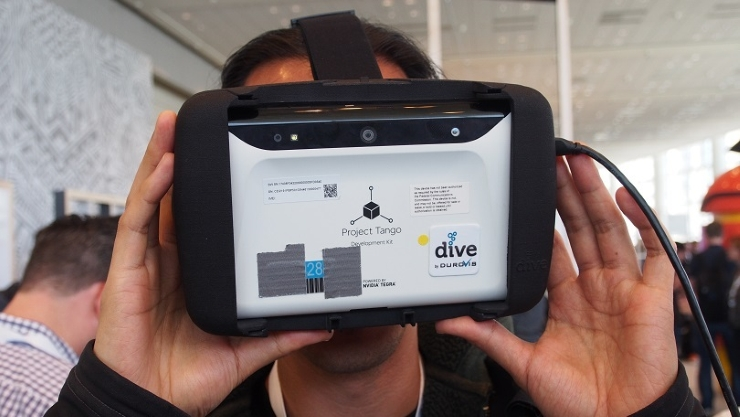
\includegraphics[width=0.9\textwidth]{images/tango.jpg}
\captionof{figure}{
Prototyp urządzenia
}
\end{center}

\paragraph{}
Google zaprezentowało również okulary do wirtualnej rzeczywistości. Jednakże był to tylko prototyp. Obecnie na rynku nie ma urządzenia dostosowanego do tego celu. Jedyną możliwością byłoby użycie Lenovo Phab Pro wraz z Google Cardboard.

\subsection{Wady i zalety}
\paragraph{}
\begin{enumerate}
	\item Project Tango jest stworzony jako kooperacja dedykowanego sprzętu oraz specjalistycznego oprogramowania, co za tym idzie wydajność urządzeń powinna być duża.
	\item Dużą wadą jest to, iż na rynku dopiero pojawił się pierwszy smartphone z obsługą projektu. Technologia wydaje się być na początkowej fazie rozwoju.
	\item Dzięki tej technologii można zrezygnować z markerów opisanych w poprzednim rozdziale. Odczucia użytkowników powinny być bardziej intuicyjne.
\end{enumerate}
